\section{Impact of heuristic placements and return policies}
\label{sec:freefloating}

 %Indeed, this solution will be our baseline to evaluate the return policies.




\subsection{Impact of heuristic charging station placements}

In this first set of experiments we evaluate which heuristic placement performs better.
Firstly, for each heuristic we consider the simple opportunistic \textit{Free Floating} car return policy, i.e., customers always return the car in the desired zone, and connect it to a charging pole if available. The goal is to check if this simple return mechanism is sustainable with electric cars, and gauge the impact of the three different heuristics for the charging station placement.
 
Fig.~\ref{fig:deathsVsZones_algorithm} shows the performance in terms of infeasible trip percentage versus an increasing percentage of charging zones, ranging from  1\% to 30\%. In Turin, this corresponds to install from 2 to 78 charging stations overall (reported in the top x-axis).
We observe notably different performances. First, the average parking time placement policy (\textit{Avg time}) performs the worst, with still 6\% of infeasible trips even when  more than 25\% of zones are equipped with charging stations. Even a simple random placement performs better (\textit{Mean rnd}, obtained as the average of 10 independent instances). The total number of parkings placement (\textit{Num parking}) reaches about 2\% of infeasible trips at 10\% coverage, reaching self-sustainability when more than 20\% of zones are equipped (no infeasible trips).

\begin{figure}[ht]
	\centering
	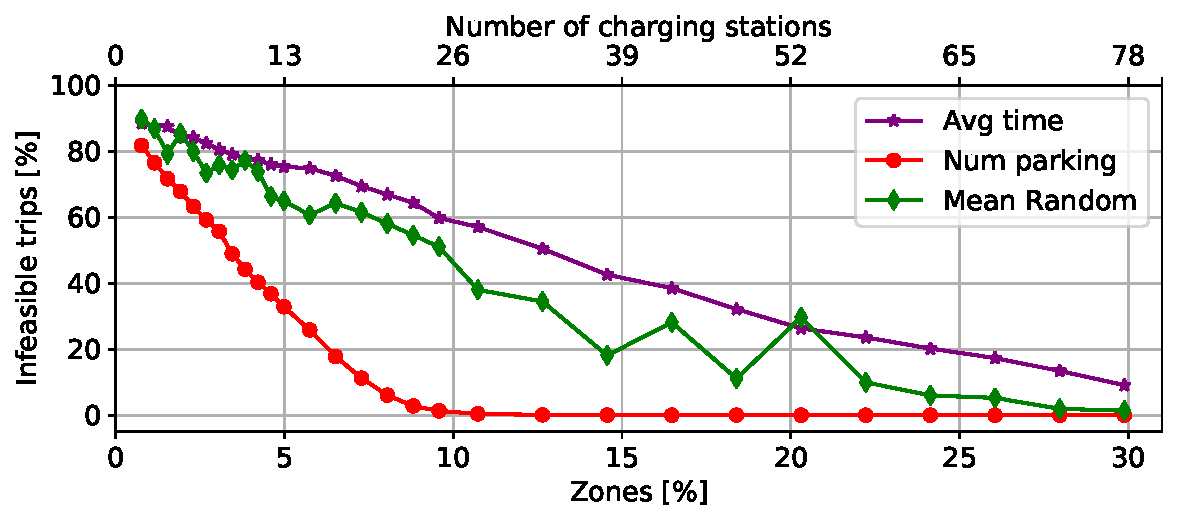
\includegraphics[width=0.9\columnwidth]{figures/Torino_FF_deaths_probs.pdf}
	\caption{Percentage of unfeasible trips as function of charging stations (percentage and number of city zones), for the different heuristic placements.}
	\label{fig:deathsVsZones_algorithm}
\end{figure}

\begin{figure}[ht]
	\centering
	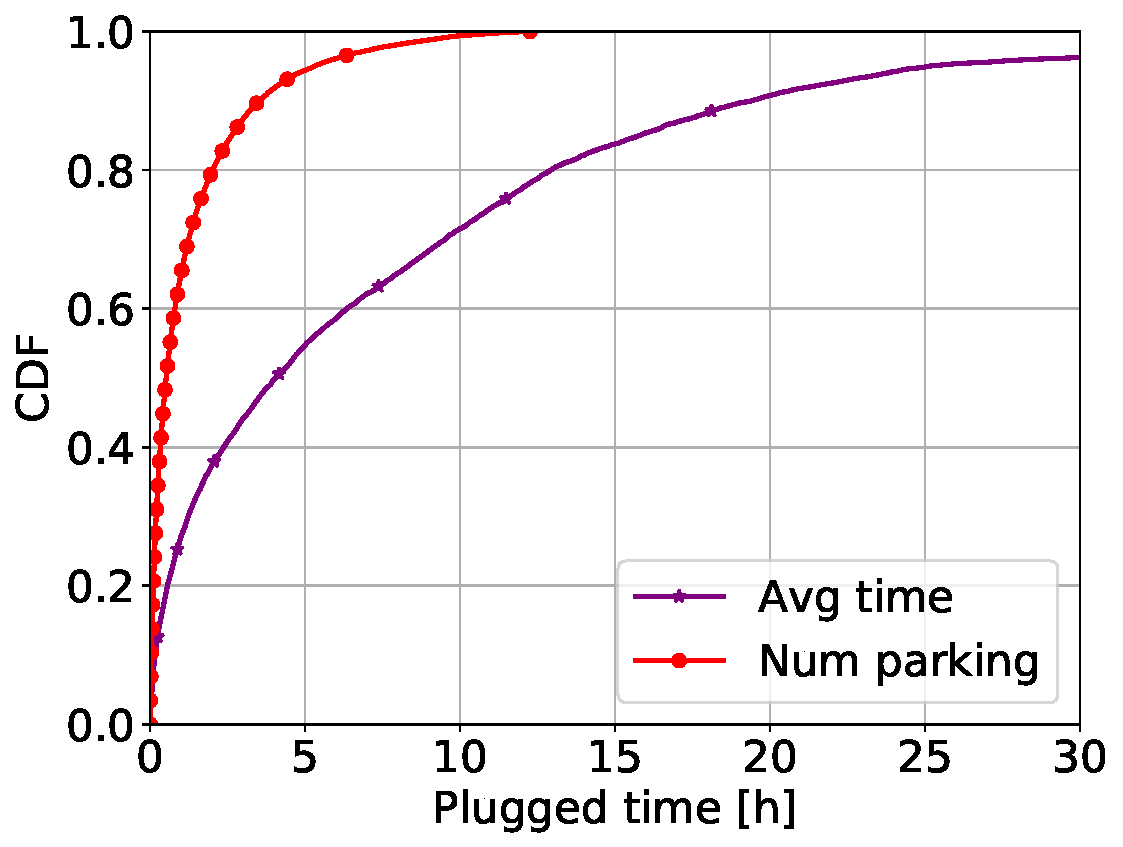
\includegraphics[width=0.5\columnwidth]{figures/CDF_parking_time_per_algorithm.pdf}
	\caption{CDF of the time spent by a car at a charging station (Z=40), for \textit{Num parking} and \textit{Avg time} placement algorithms. }
		\label{fig:CDF_parking_time_per_algorithm}
\end{figure}

The intuition of why such a striking difference is given by the different properties of areas where the heuristics place charging stations. \textit{Avg time} placement favours peripheral zones where few trips ends, and where cars stay parked for long time (see Fig. \ref{fig:hm_avg-time}). On the contrary, \textit{Num parking} favours city centre areas, where cars frequently are parked for short time (see Fig. \ref{fig:hm_max-parking}). Indeed, in the whole simulation, for $Z=40$ ($\approx 15\%$ of zones), only 7\,430 charges have been recorded for \textit{Avg time}, compared with 47\,628 charges of the \textit{Num parking}.
Even if plugged time is shorter, the \textit{Num parking} policy allows the cars to charge the (little) energy consumed during the (short) trips.
Moreover, as shown in Fig. \ref{fig:CDF_parking_time_per_algorithm} the \textit{Avg time} placement generates much longer plugged times, often much longer than the time needed for a full charge. Therefore, many cars occupy the charging poles when they are already charged, preventing other cars to use those poles and increasing the number of infeasible trips. 

In a nutshell the best approach among these three heuristics is to place charging stations in the central areas, in which the parkings last less but are more frequent. For this reason, we will use the \textit{Num parking} placement algorithm as best heuristic for the remaining of the paper.



\subsection{Impact of return policy}

We now investigate the impact of the three different return policies. We quantify the implications of forcing customers to return the car to a different zone than the desired one, when the battery is below a critical level (i.e., below the percentage threshold $\alpha=25\%$ of full battery capacity).

We focus again on the infeasible trip percentage with respect to the charging station coverage.
Fig. \ref{fig:deathsVsZones_policy} shows results, with \textit{Num Parking} placement. \textit{Needed} and \textit{Hybrid} policies perform much better than the opportunistic \textit{Free Floating}.
In details, \textit{Hybrid} and \textit{Needed} guarantee to successfully conclude all trips with just $Z=11$ and $Z=15$ charging zones, respectively (4.2\% and 5\% of the zones), while \textit{Free Floating} reaches this goal only at $Z=60$  (23\% of zones).
In a nutshell, adopting a policy which mandates customers to charge the cars when battery level gets low drastically reduces the number of infeasible trips, even with a handful of  charging stations.

\begin{figure}[ht]
	\centering
	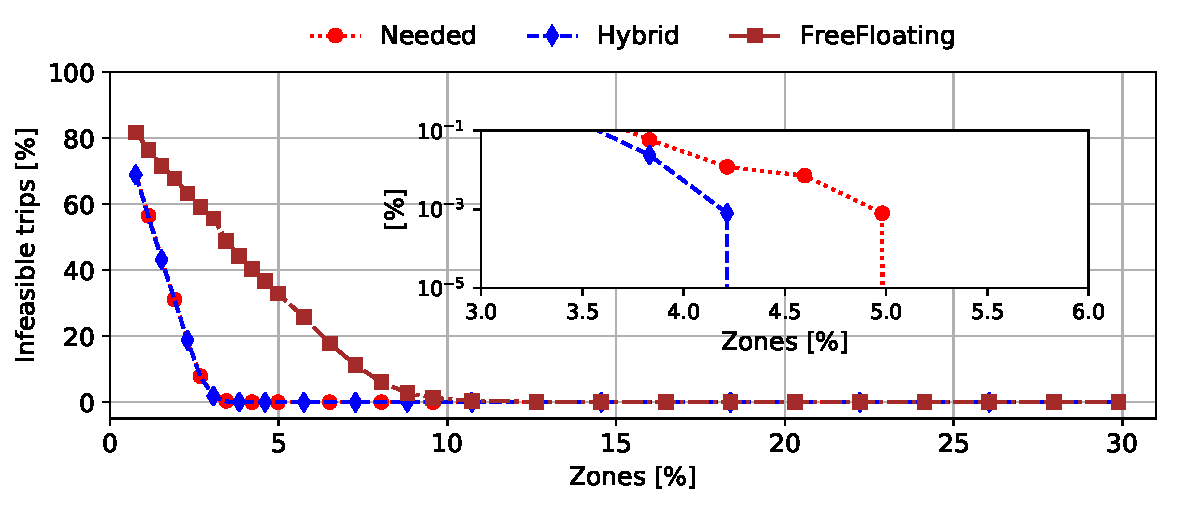
\includegraphics[width=0.95\columnwidth]{figures/Torino_H_N_FF_deaths_probs.pdf}
	\caption{Percentage of infeasible trips for different zone coverage percentage analysing the return policies. The inset highlights where the infeasible trips go to 0.}
	\label{fig:deathsVsZones_policy}
\end{figure}

\begin{figure}[ht]
    \centering     
    \subfloat[][Percentage of trips ending with a charge.]
    {
        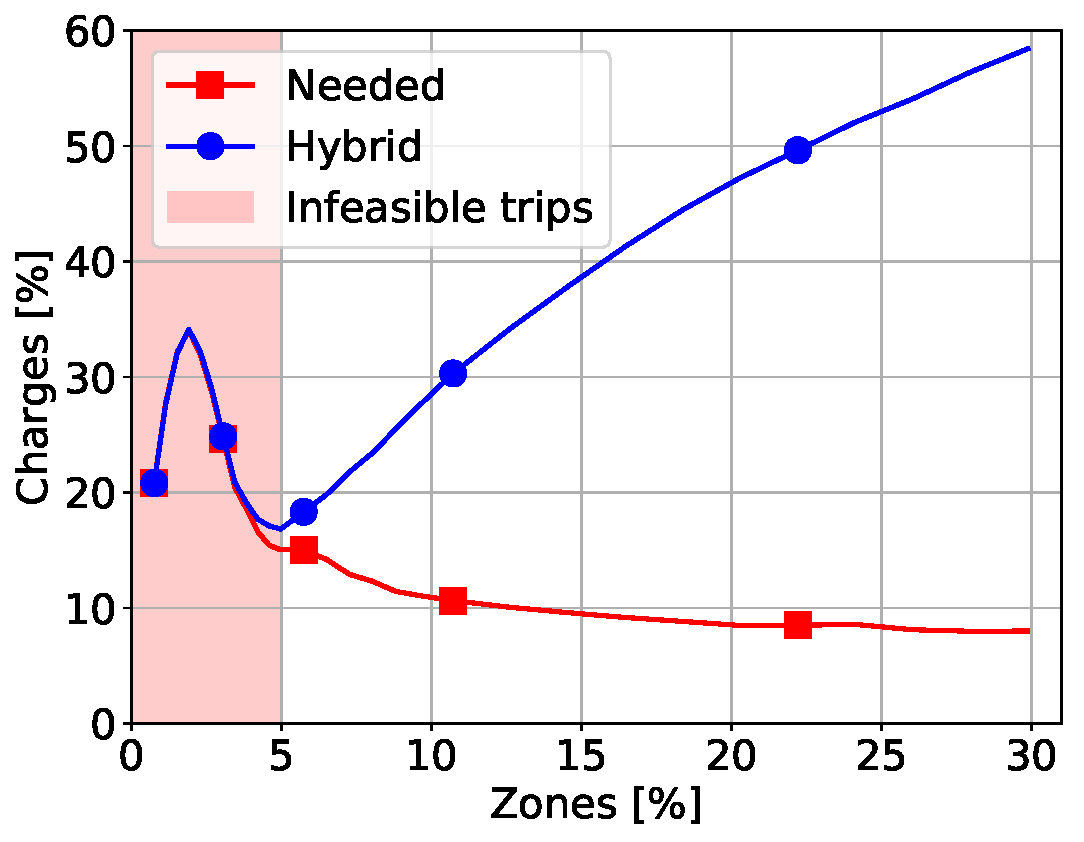
\includegraphics[width=0.45\textwidth]{figures/Taormina_Torino_AmountRechargePerc.pdf}
        \label{fig:recharge_perc}
    }
    \subfloat[][Rerouted trips percentage.]
    {
        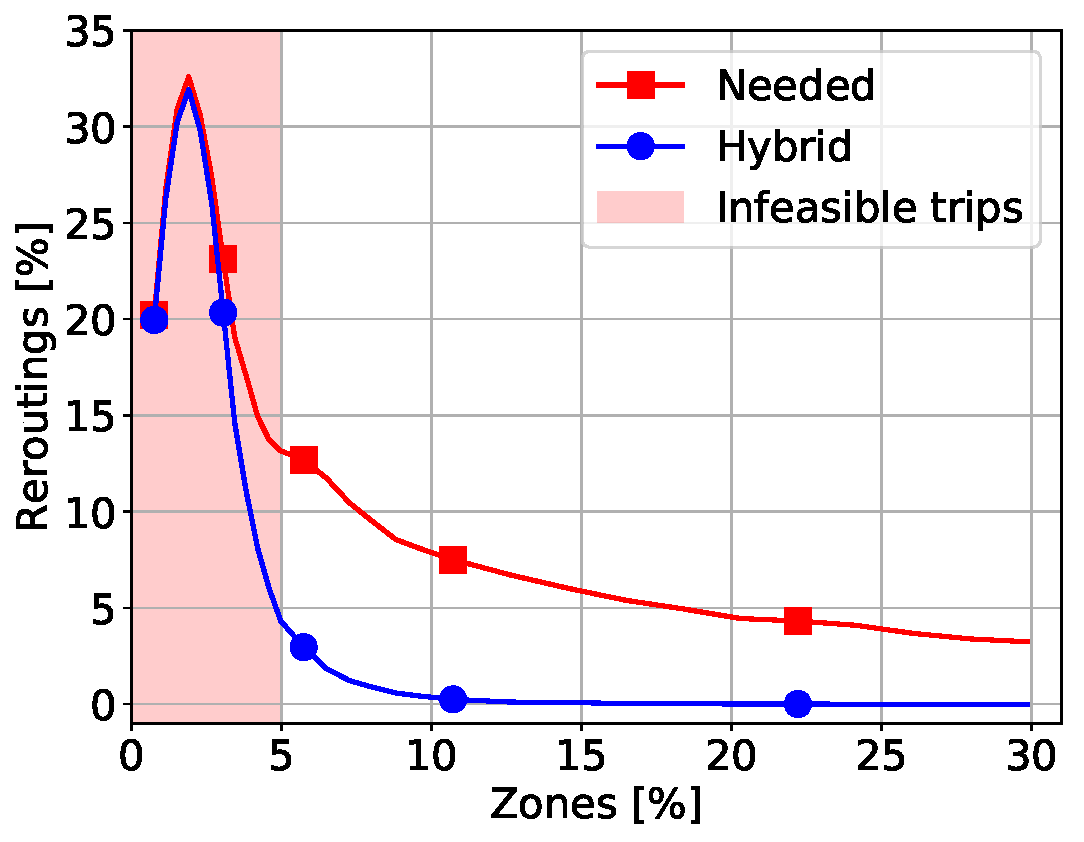
\includegraphics[width=0.45\textwidth]{figures/Taormina_Torino_ReroutePerc.pdf}
        \label{fig:reroute_perc}
    }
    \subfloat[][Walked distance, averaged over all trips.]
    {
        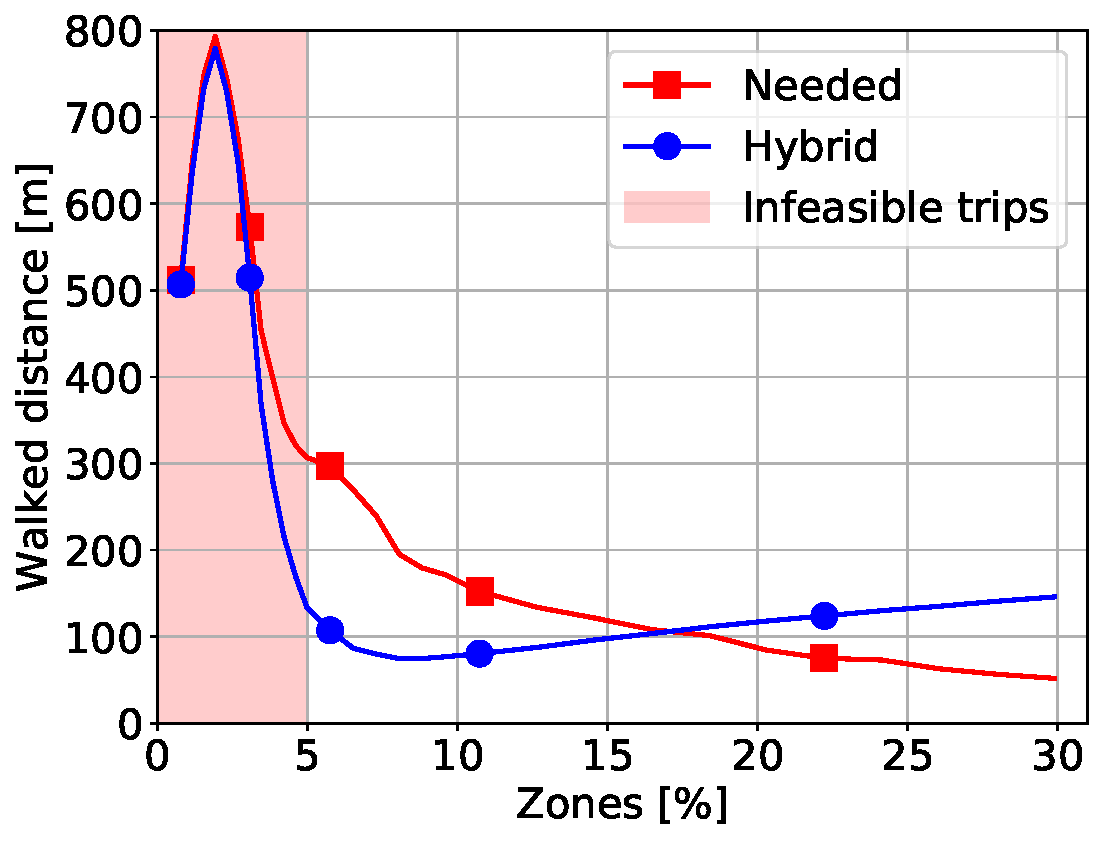
\includegraphics[width=0.45\textwidth]{figures/Taormina_Torino_TravelWithPenlaty.pdf}
        \label{fig:global_weighted_distance}
    }
    
    \caption{Metrics of interests when comparing Hybrid and Needed return policy (Max parking placement adopted).}
    \label{}
\end{figure}

\subsubsection{Customers' discomfort}
%questa e' una subsection della scelta della policy, non una a parte

Forcing customers to charge batteries, even at cost or rerouting them has clearly an impact on their comfort. Indeed, forcing a customer to park in a charging station can be annoying, because of the burden of reach the charging station, and losing time to plug to and unplug the car from the pole. Even worse, rerouting customers to the closest zone for charging increases the distances they have to walk to reach the desired destination. 

Fig. \ref{fig:recharge_perc} reports the percentage of trips that end by charging the car. Shaded area highlights the infeasible region, where the lack of charging zones create artefacts. Focusing on the feasible region instead, the two curves start with similar values, but then they diverge. Interestingly, the percentage of charges decreases for the \textit{Needed} policy, getting as low as 8\%. This suggests a better usage of each single charge, i.e., the battery fills up and does not need frequent charges. 
%This happens when few stations are present and all of them can be occupied. Hence some cars will not be charged despite they would need to. 
Conversely, the \textit{Hybrid} policy increases steadily the fraction of trips where customers have to plug to a pole. This because the higher $Z$, the higher the probability of ending the trip in a zone with a free charging pole.

Fig. \ref{fig:reroute_perc} represents the rerouting percentage in function of charging stations coverage.
Rerouting probability decreases as expected: the more the stations are, the more likely customers find a charging station at their desired final zone. Yet, the two policies have different performance. The \textit{Hybrid} policy is less likely to reroute customers. In fact, by opportunistically connecting the car to a charging pole if available, the average battery charge is high, thus decreasing the rerouting probability. With more than 7\% of charging zones, the percentage of rerouting is already lower than 1\% for \textit{Hybrid} policy.
In a nutshell, \textit{Hybrid} policy significantly reduces the number of times the customer has to drive to a charging station in a different zone than the desired one. However, it increases the number of times the customer parks at a charging station and has to plug the car to the pole. Therefore, one must be cautious when weighting these results and designing return policies which impact the customers' comfort. 

Whenever the system forces a customer to park the car in a charging station, customers may be routed far from their desired destination. If the charging station is not in the final destination zone, the customer has to walk by at least 500\,m to reach their final destination. Even in case the charging station is found inside the final zone, the customer will have to park at the charging station, instead of the desired destination. 
For this reason, we evaluate the average distance the customers have to walk to reach their actual final destination. 
In details, when the customers suffer rerouting, we evaluate the actual distance between the charging station and the final destination. When they end in a charging zone and plug the car, we count an average distance of 150\,m. Finally, if the customers do not charge the car, we assume they arrived at their final destination directly.

Results are shown in Fig. \ref{fig:global_weighted_distance}.
Consider the feasible region. The \textit{Needed} policy exhibits a decreasing trend (from 280 m to 60 m). On the contrary, the \textit{Hybrid} policy first exhibits a decrease (minimum of 50 m at 8\% of charging zones), but then it slowly increases till it overtakes the \textit{Needed} policy. 
This is due to the fact that with few charging stations (6-15\%) the number of charges is limited ($<$ 30\%, see Fig. \ref{fig:recharge_perc}) by the availability of charging stations. Instead, when this number grow, the opportunistic \textit{Hybrid} policy 
forces the customer to walk more times within the ending zone.
To this extent, the \textit{Needed} policy performs better. 

Even if the values of walked distances seem very small, remember that they are averaged over all trips. Restricting to the few long walks due to rerouting (not reported for the sake of brevity), the walked distance that we observe ranges from 2\,200\,m to 1\,500\,m, with similar behaviours for the two policies. 
Recall that the charging station placement algorithm likely places stations mainly in the city centre. Therefore, the charging stations are concentrated in a small area, so that rerouting from the suburbs significantly affects the walked distance when rerouted. This gives hope for further optimisation, as we will see in the next section.

Given the very few rerouting of the \textit{Hybrid policy}, one can envision a system which directly takes care of those very few cars that need a battery charge, i.e. by relocating vehicles. For instance less than 3 cars per day would need to be relocated with 15\% coverage or higher.

In summary, with \textit{Hybrid} policy, less than 15\% of zones guarantees all trips to be feasible, reduces the walked distance, asks for few rerouting events, at the cost of moderately high percentage of times (40\%) customers are asked to charge the battery.




